% Modified based on Xiaoming Sun's template and https://www.overleaf.com/latex/templates/cs6780-assignment-template/hgjyygbykvrf

\documentclass[a4 paper,12pt]{article}
\usepackage[inner=2.0cm,outer=2.0cm,top=2.0cm,bottom=2.0cm]{geometry}
\linespread{1.1}
\usepackage{setspace}
\usepackage[rgb]{xcolor}
\usepackage{verbatim}
\usepackage{subcaption}
\usepackage{fancyhdr}
\usepackage{fullpage}
\usepackage[colorlinks=true, urlcolor=blue, linkcolor=blue, citecolor=blue]{hyperref}
\usepackage{booktabs}
\usepackage{amsmath,amsfonts,amsthm,amssymb}
\usepackage[shortlabels]{enumitem}
\usepackage{setspace}
\usepackage{extramarks}
\usepackage{soul,color}
\usepackage{graphicx,float,wrapfig}
\newenvironment{breakablealgorithm}
  {% \begin{breakablealgorithm}
   \begin{center}
     \refstepcounter{algorithm}% New algorithm
     \hrule height.8pt depth0pt \kern2pt% \@fs@pre for \@fs@ruled
     \renewcommand{\caption}[2][\relax]{% Make a new \caption
       {\raggedright\textbf{\ALG@name~\thealgorithm} ##2\par}%
       \ifx\relax##1\relax % #1 is \relax
         \addcontentsline{loa}{algorithm}{\protect\numberline{\thealgorithm}##2}%
       \else % #1 is not \relax
         \addcontentsline{loa}{algorithm}{\protect\numberline{\thealgorithm}##1}%
       \fi
       \kern2pt\hrule\kern2pt
     }
  }{% \end{breakablealgorithm}
     \kern2pt\hrule\relax%
   \end{center}
  }
\makeatother
\newtheoremstyle{definitionstyle}
  {3pt} % Space above
  {3pt} % Space below
  {\normalfont} % Body font
  {} % Indent amount
  {\bfseries} % Theorem head font
  {} % Punctuation after theorem head
  { } % Space after theorem head
  {} % Theorem head spec (can be left empty, meaning `normal`)

\theoremstyle{definitionstyle}
\newtheorem{defn}{Definition}
\newtheorem{thm}{Theorem}
\newtheorem{lem}{Lemma}
\newtheorem{statement}{Statement}
% \newtheorem{proof}{Proof}
\usepackage{framed}
\newenvironment{framedminipage}
    {\begin{framed}\begin{minipage}{0.9\textwidth}}
    {\end{minipage}\end{framed}}
\newcommand{\homework}[3]{
	\pagestyle{myheadings}
	\thispagestyle{plain}
	\newpage
	\setcounter{page}{1}
	\noindent
	\begin{center}
		\framebox{
			\vbox{\vspace{2mm}
				\hbox to 6.28in { {\bf Deep Learning \hfill} {\hfill {\rm #2} {\rm #3}} }
				\vspace{4mm}
				\hbox to 6.28in { {\Large \hfill #1  \hfill} }
				\vspace{3mm}}
		}
	\end{center}
	\vspace*{4mm}
}
\newcommand\numberthis{\addtocounter{equation}{1}\tag{\theequation}}

\begin{document}
\homework{HW1}{2024011303}{Liu Hanzuo}
\section*{True or False}
\paragraph{P1}No, the greatest advantage of residual connection is that it prevent the model from exploding or vanishing gradients.
\paragraph{P2}Yes, though it is not recommended to connect batchnorm and dropout layers straightly, we may use them in the same network: such as use batchnorm is convolutional layers while use dropout in fully connected layers.
\paragraph{P3}No, in fact, layer norm is a special case of group norm, which calculates the normalization on channel levels (group norm consider several channels as a group), however, batch norm takes batch to normalize. Thus batch norm is not a special case of layer norm.

\section*{Q\&A}
\paragraph{P4}Note that the following equation holds:
\[
    f(y)-f(x)=\int_0^1 \nabla f\left(x+t(y-x)\right)^T(y-x)dt
\]
\[
    \le\nabla f(x)^T(y-x)+\int_0^1\left(\nabla f\left(x+t(y-x)\right)-\nabla f(x)\right)^T(y-x)dt
\]
\[
    \le \nabla f(x)^T (y-x)+\int_0^1 Lt\|y-x\|^2dt=\nabla f(x)^T(y-x)+\frac{L}{2}\|y-x\|^2
\]
Thus, to conclude,
\[
    f(y)\le f(x)+\nabla f(x)^T(y-x)+\frac{L}{2}\|y-x\|^2
\]
\paragraph{P5}Here we show two boundaries of inequalities
\begin{framedminipage}
\begin{thm}
\[
	f(x^{k+1})\le f(x^k)-\frac{1}{2L}\|\nabla f(x^k)\|^2
\]
\end{thm}
\end{framedminipage}
\begin{proof}
From descent lemma we have showed,
\[
	f(x^{k+1})\le f(x^k)+\nabla f(x^k)(x^{k+1}-x^k)+\frac{L}{2}\|x^{k+1}-x^k\|^2
\]
\[
	=f(x^k)-\eta\|\nabla f(x^k)\|^2+\frac{L}{2}\eta^2\|\nabla f(x^k)\|^2=f(x^k)-\frac{1}{2L}\|\nabla f(x^k)\|^2
\]
\end{proof}
\begin{framedminipage}
\begin{thm}
\[
	\|\nabla f(x^k)\|^2\ge 4\mu\left(f(x^k)-f(x^*)\right) 
\]
\end{thm}
\end{framedminipage}
\begin{proof}
\[
	f(x^*)\ge f(x^k)+\nabla f(x^k)^T(x^*-x^k)+\mu\|x^*-x^k\|^2\ge f(x^k)-\frac{1}{4\mu}\|\nabla f(x^k)\|^2
\]
thus we have
\[
	\|\nabla f(x^k)\|^2\ge 4\mu\left(f(x^k)-f(x^*)\right) 
\]
\end{proof}
Come back to the initial question, we have:
\[
	f(x^{k+1})-f(x^*)\le f(x^k)-f(x^*)-\frac{1}{2L}\|\nabla f(x^k)\|^2
\]
\[
	\le f(x^k)-f(x^*)-\frac{2\mu}{L}\left(f(x^k)-f(x^*)\right)=(1-\frac{2\mu}{L})\left(f(x^k)-f(x^*)\right)
\]
Thus we have
\[
	\mu\|x^k-x^*\|^2\le f(x^k)-f(x^*)\le(1-\frac{2\mu}{L})^k(f(x^0)-f(x^*))\le (1-\frac{2\mu}{L})^kL\|x^0-x^*\|^2
\]
bring $\|x^k-x^*\|\le\epsilon$ in this ineuqality, we only need to guerantee that
\[
	(1-\frac{2\mu}{L})^k\le\frac{\epsilon^2\mu}{LR^2}
\]
We calculate $k$ out, we have
\[
	k\ge\frac{\log \frac{\epsilon^2\mu}{LR^2}}{\log(1-\frac{2\mu}{L})}\approx\frac{L}{2\mu}\log\frac{LR^2}{\epsilon^2\mu}\in O(\frac{L}{\mu}\log\frac{R}{\epsilon})
\]
Note that here we use the approximation that
\[
	\log(1+x)\approx x,\forall x\to 0
\]
\paragraph{P6}
note that the gradient of each function integral is listed below:
\[
  \nabla f(x)=\begin{cases}
    25x \text{ if }x<1\\
    x+24 \text{ if }1\le x<2\\
    25x-24 \text{ if }2\le x
  \end{cases}
\]
The update step is listed as below:
\[
  x^{k+1}=\begin{cases}
    -\frac{4}{3}x^k-\frac{4}{9}x^{k-1}\text{ if }x^k<1\\
    \frac{4}{3}x^k-\frac{4}{9}x^{k-1}-\frac{8}{3}\text{ if }1\le x^k<2\\
    -\frac{4}{3}x^k-\frac{4}{9}x^{k-1}+\frac{8}{3}\text{ if }2\le x^k
  \end{cases}
\]

\begin{figure}[H]
  \centering
  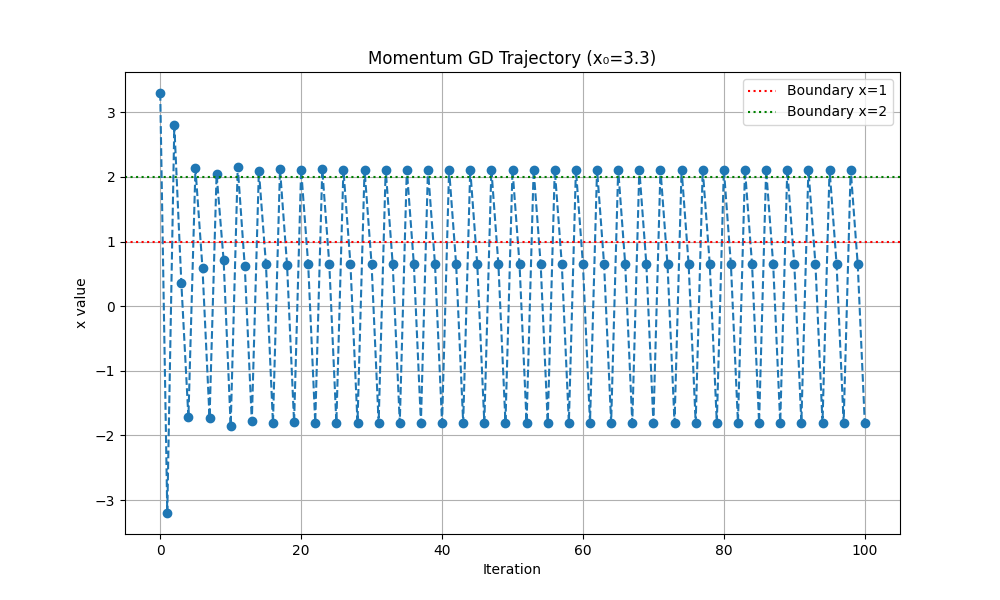
\includegraphics[width=0.8\textwidth]{momentum_gd.png}
  \caption{Momentum Method}
\end{figure}
\begin{framedminipage}
  \begin{statement} For any $k\ge 2$, we have other $x^k$ diverges, other we have:
  \[
    x^k\in\begin{cases}
      (2,\infty)\text{ if }k\mod 3=2\\
      (-\infty,1)\text{ if }k\mod 3=0,1
    \end{cases}
  \]
  \end{statement}
\end{framedminipage}
The non-convergence proof can be reduced to the proof of this statement.
\begin{proof}
for $k\mod 3=2$, the recurrence formula could be written as 
\[
  x^{k+3}=-\frac{4}{3}x^{k+2}-\frac{4}{9}x^{k+1}
\]
\[
  =\frac{4}{3}x^{k+1}+\frac{16}{27}x^k
\]
\[
  =-\frac{32}{27}x^k-\frac{16}{27}x^{k-1}+\frac{32}{9}
\]
The characteristic polynomial is 
\[
  f(t)=t^4+\frac{32}{27}t+\frac{16}{27}
\]
Solve the equation that $f(t)=0$, we have the roots are 
\[
  x_1=x_2=-\frac{2}{3},x_3=\frac{2-2\sqrt{2}i}{3},x_4=\frac{2+2\sqrt{2}i}{3}
\]
Thus, the General form formuls could be written as (coefficient before $x_3$ and $x_4$ are same due to the conjugate roots)
\[
  x^k=(-\frac{2}{3})^k(A+Bk)+C(\frac{2-2\sqrt{2}i}{3})^k+C(\frac{2+2\sqrt{2}i}{3})^k-\frac{2208}{1225}
\]
if $C!=0$, then $(-\frac{2}{3})^k(A+Bk)$ converge and $C(\frac{2-2\sqrt{2}i}{3})^k+C(\frac{2+2\sqrt{2}i}{3})^k$ diverge, then $x^k$ diverge.\\
if $C=0$, then $x^k=(-\frac{2}{3})^k(A+Bk)-\frac{2208}{1225}$, thus $x^k$ converges to $-\frac{2208}{1225}$. Thus, other cases also converge:
\[
  x^k\to\begin{cases}
    \frac{2592}{1225}\text{ if }k\mod 3=2\\
    \frac{792}{1225}\text{ if }k\mod 3=0\\
    -\frac{2208}{1225}\text{ if }k\mod 3=1
  \end{cases}
\]
To conclude, the statement holds! And the proof ends.
\end{proof}
\paragraph{P7}
We could simplify the inequality of 
\[
  \|x_{k+1}-x^*\|\le C\|x_k-x^*\|^2
\]
to 
\[
  \log\|x_{k+1}-x^*\|+\log C\le 2\left(\log C+\log\|x_k-x^*\|\right)
\]
thus we have
\[
  \log \|x_k-x^*\|+\log C\le 2^k\left(\log\|x_0-x^*\|+\log C\right)\le 2^k \log\delta C
\]
thus we have
\[
  \|x_k-x^*\|\le (\delta C)^{2^k}/C
\]
we only need to guerantee that $(\delta C)^{2^k}/C\le\epsilon$, thus we have
\[
  2^k\log\delta C\le\log\epsilon C
\]
\[
  k\ge\log{\frac{\log\epsilon C}{\log\delta C}}
\]
\paragraph{P8}
let's say that $\nabla^f$ is $l-$lipschitz and $\nabla f$ is $l$-smooth. Note that
\begin{framedminipage}
  \begin{thm}
  \[
    \|\nabla f(x^*)-\nabla f(x^k)-\nabla^2 f(x^k)(x^*-x^k)\|\le\frac{l}{2}\|x^*-x^k\|^2
  \]
  \end{thm}
  \end{framedminipage}
\[
  \|x^{k+1}-x^*\|=\|x^k-x^*-\frac{\nabla f(x^k)}{\nabla^2 f(x^k)}\|=\|(\nabla^2 f(x^k))^{-1}\left(\nabla^2f(x^k)(x^k-x^*)-\nabla f(x^k)\right)
\]
\[
  \le\frac{l}{2}\|\nabla^2 f(x^k)\|^{-1}\|x^k-x^*\|^2\le\frac{l}{2\mu}\|x^k-x^*\|^2
\]
Utilize the conclusion from \textbf{P7}, thus we get the conclusion that the newton-method is quadratically convergent.
\paragraph{P9}
\[
  Var(Z_i^l)=Var\left(\sum_j W_{i,j}^l ReLU(Z_j^{l-1})\right)
\]
\[
  =\sum_j \mathbb{E}\left((W_{i,j}^l)^2ReLU(Z_j^{l-1})^2\right)-\left(\mathbb{E}\left(W_{i,j}^lReLU(Z_{j}^{l-1})\right)\right)^2
\]
\[
  =\sum_j Var(W_{i,j}^l)\mathbb{E}\left(ReLU(Z_j^{l-1})^2\right)
\]
\[
  =\frac{1}{2}\sum_j Var(W_{i,j}^l)\mathbb{E}(Z_{j}^{l-1})^2=\frac{1}{2}Var(W_{i,j}^l)\sum_j Var(Z_j^{l-1})=\frac{1}{2}Var(W^l)Var(Z^{l-1})
\]
to make them have same variance, we need to make sure that
\[
  Var(Z^l)=h_lVar(Z_i^l)
\]
thus we have
\[
  Var(W^l)=\frac{2}{h_l}
\]
and the initial statement holds.
\end{document} 
